\chapter{Client and Tooling Architecture}
\label{ch:frontend-architecture}

The product has no web or mobile user interface of its own. ``Frontend'' here
means the two developer-facing surfaces: the command-line interface and the VS Code
extension. Both are thin orchestration layers over the shared engine documented in
Chapter~\ref{ch:software-architecture}.

\section{Surface comparison}

\begin{longtable}{p{3.4cm}p{4.6cm}p{5.8cm}}
\caption{CLI versus VS Code extension}\\
\toprule
\textbf{Aspect} & \textbf{CLI} & \textbf{VS Code extension} \\
\midrule

Package & \texttt{@expo-snips/cli} & \texttt{expo-snippets} \\
Version & 0.1.0 & 0.1.3 \\
Entry point & \texttt{src/index.ts} (commander) & \texttt{src/extension.ts} (\texttt{activate}) \\
Engine & imported \texttt{@expo-snips/core} & same, bundled by esbuild \\
Discovery & \texttt{list}; interactive select in \texttt{add} & completion, Quick Pick, status bar \\
Option resolution & prompts when unresolved & detection plus settings defaults, never prompts \\
Variant selection & \texttt{--variant} flag & Quick Pick when variants exist \\
Update and status & implemented & \textbf{not implemented} \\
Project root & \texttt{process.cwd()} & first workspace folder \\
Dependency install & \texttt{execSync}, blocking, inherited stdio & terminal command, non-blocking \\
Offline catalog & embedded at build & embedded at build \\
Registry fetch & every invocation (no cache) & cached 5 minutes with back-off \\
Failure reporting & coloured stderr, exit code & VS Code error/information notifications \\
\bottomrule
\end{longtable}

\section{Command-line interface architecture}

The CLI is a single-process program. Startup cost is the commander registration
plus a static module import of the embedded catalog.

\begin{itemize}
  \item \textbf{Parsing:} commander defines the program and five subcommands.
  \item \textbf{Interaction:} \texttt{prompts} drives the select prompts in
        \texttt{add} and the confirm prompt in \texttt{update}.
  \item \textbf{Presentation:} \texttt{chalk} colours informational (cyan), success
        (green), warning (yellow) and error (red) output.
  \item \textbf{Exit codes:} 0 on success; 1 on any handled error
        (\texttt{process.exitCode = 1}).
\end{itemize}

\section{VS Code extension architecture}

\begin{figure}[H]
\centering
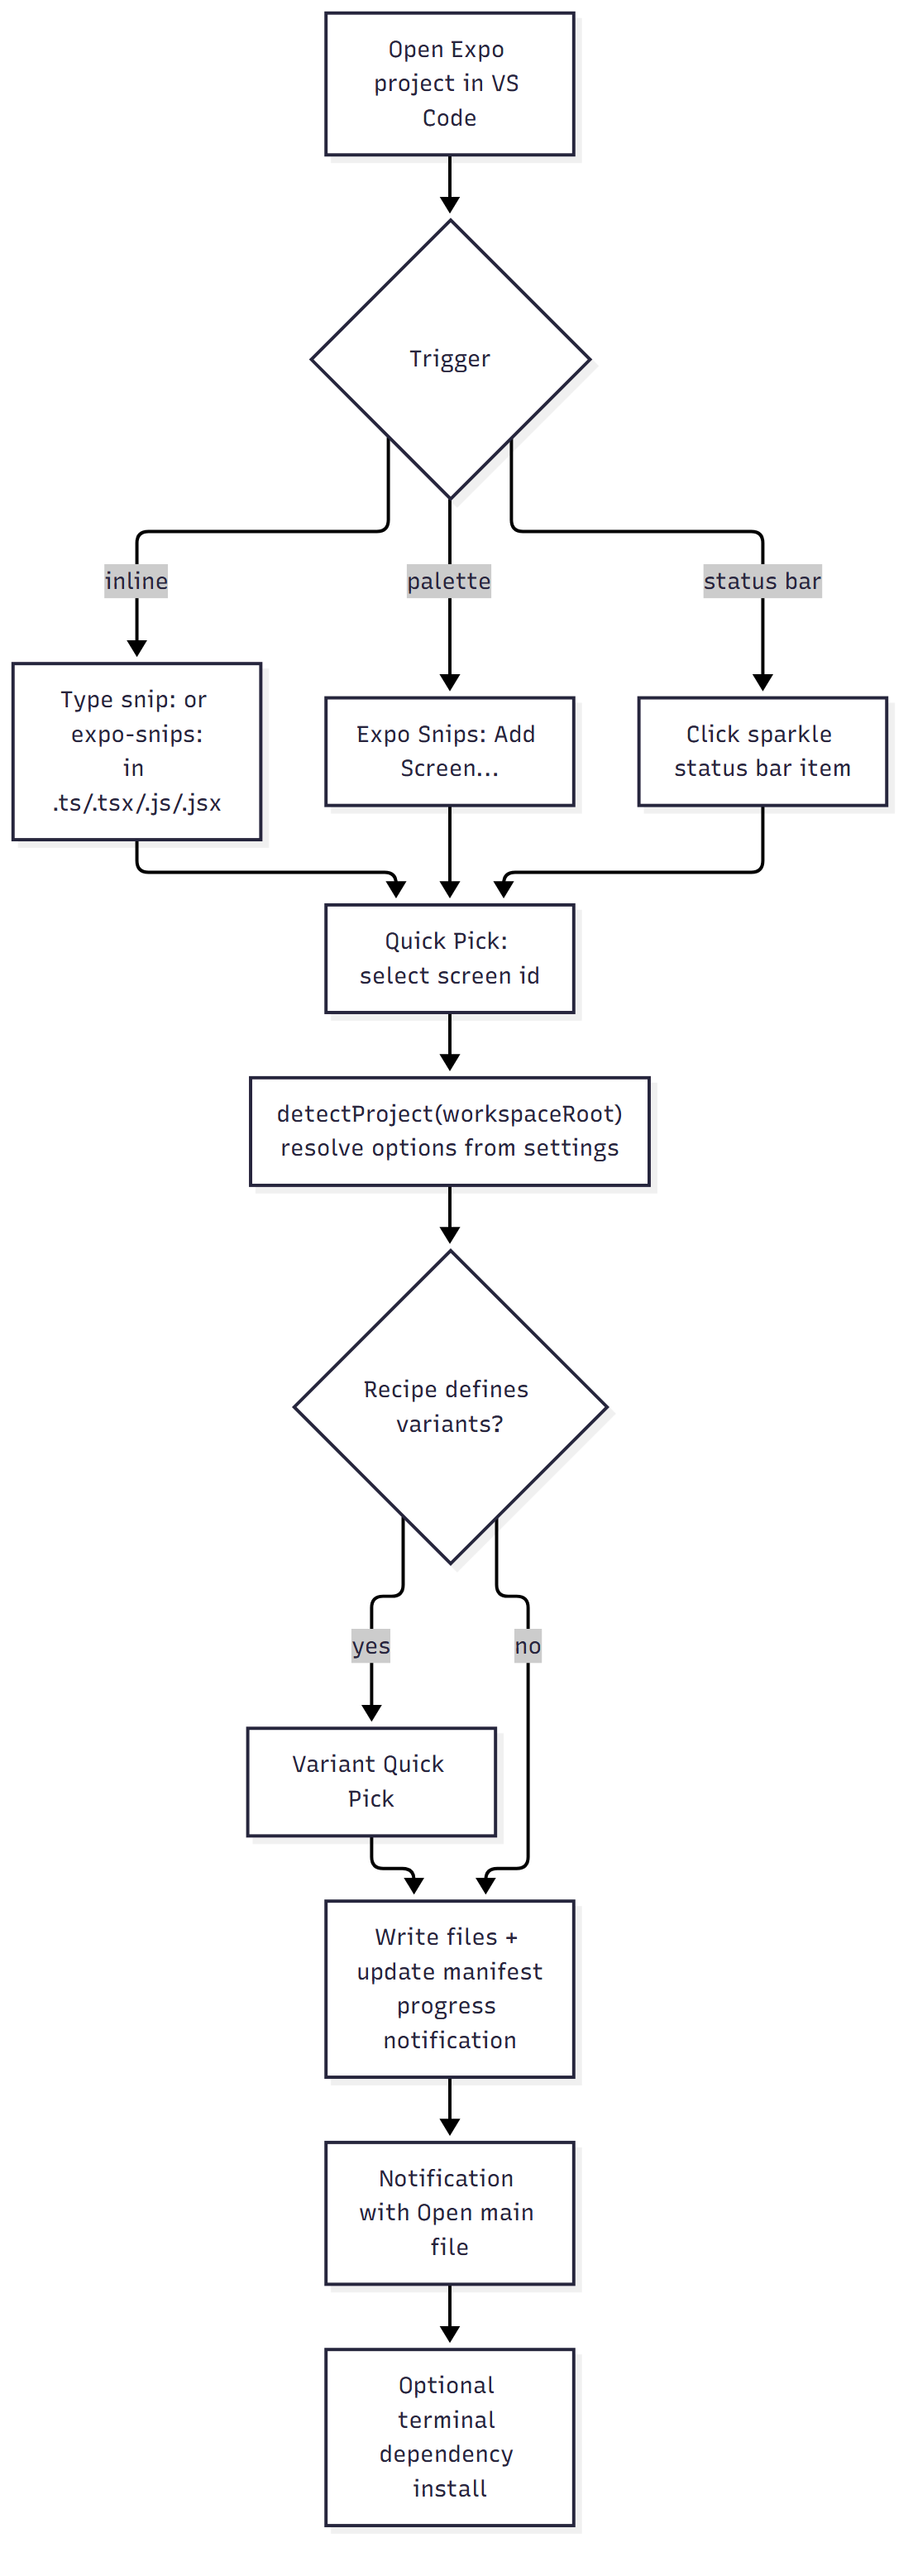
\includegraphics[width=0.95\textwidth]{diagrams/user-flow-vscode.png}
\caption{VS Code extension interaction flow}
\label{fig:user-flow-vscode}
\end{figure}

\subsection*{Activation}

The extension declares four activation events
(\texttt{packages/vscode-extension/package.json}, lines 74--80):
\texttt{onCommand:expo-snips.addScreen} and \texttt{onLanguage:} for TypeScript,
TypeScript React, JavaScript and JavaScript React. It therefore activates when a
relevant file is opened or when the command is invoked first.

\subsection*{Surfaces}

\begin{enumerate}
  \item \textbf{Inline completion.} Registered for the four language ids and
        triggered on the \texttt{:} character. The provider inspects the text before
        the cursor; on a match it produces one completion item per catalog entry,
        labelled with the recipe id and described with the recipe name,
        documentation and tags. Because \texttt{insertText} is empty and the item
        carries a command, selecting it triggers generation rather than inserting
        text.
  \item \textbf{Command palette.} \texttt{Expo Snips: Add Screen...} (declared in
        \texttt{contributes.commands}) opens a Quick Pick with matching on
        description enabled.
  \item \textbf{Status bar.} A right-aligned item at priority 100, showing the
        \texttt{sparkle} codicon and the text ``Expo Snips'', tooltip ``Add an Expo
        Snip screen'', bound to the add-screen command.
  \item \textbf{Post-generation notification.} Reports the recipe name and file
        count and offers a single action, ``Open main file'', which opens the first
        written path.
\end{enumerate}

\subsection*{Command identifiers}

\begin{table}[H]
\centering
\caption{VS Code command identifiers}
\begin{tabular}{p{6cm}p{7.6cm}}
\toprule
\textbf{Command id} & \textbf{Declared in \texttt{contributes.commands}?} \\
\midrule
\texttt{expo-snips.addScreen} & yes \\
\texttt{expo-snips.generateFromCompletion} & no --- registered at runtime only \\
\bottomrule
\end{tabular}
\end{table}

The second command is intentionally internal (it exists so completion items can
dispatch a generation). Because it is not contributed, it is invisible in the
command palette, which is the desired behaviour.

\subsection*{Progress and feedback}

Generation runs inside \texttt{vscode.window.withProgress} with a notification
location and the title ``Expo Snips: generating \{recipe name\}...'', so file writes
and primitive resolution are covered by a progress indicator.

\section{Shared client concerns}

\subsection*{Project detection}

Both clients implement the same five probes. The implementations are separate
files with near-identical bodies (\texttt{cli/src/utils/detectProject.ts} and
\texttt{vscode-extension/src/project.ts}). Only \texttt{dependencies} is inspected;
packages present solely under \texttt{devDependencies} are not detected.

\subsection*{Registry access}

Both clients:
\begin{itemize}
  \item keep an embedded catalog as the default;
  \item accept a base URL from different sources (flag/env for the CLI, a setting
        for the extension);
  \item normalise the base by trimming and stripping trailing slashes;
  \item use a 10-second abort timeout;
  \item fall back to the embedded catalog on any failure.
\end{itemize}

Differences: the extension caches and backs off; the CLI does not cache.

\subsection*{Manifest}

Both clients read and upsert \texttt{.expo-snips.json} with the same shape and the
same upsert key. The extension does not implement version bumping because it has
no update command.

\section{Presentation layer of generated screens}

Generated screens are React Native components. Their structure --- components,
styles, states and interactions --- is documented as a design system in
Chapter~\ref{ch:design-system}. The templates consistently follow a
presentational split:

\begin{itemize}
  \item a \textbf{screen} file (route-level, handles layout, safe area and
        keyboard avoidance);
  \item a \textbf{form or list item component} (encapsulates field or row
        rendering);
  \item a \textbf{hook} where async behaviour exists (for example
        \texttt{useLogin}, \texttt{useRegister});
  \item inline sample data constants (for example \texttt{stats},
        \texttt{upcoming}, product arrays) that the developer replaces.
\end{itemize}

This is IMPLEMENTED and observable across \texttt{packages/registry/templates/**}.
